%%%%%%%%%%%%%%%%%%%%%%%%%%%%%%%%%%%%%%%%%%%%%%%%%%%%%%%%%%%%%%%%%%%%%%%%%%%%%%
% $Id: mini_aes.tex,v 1.2 2005-12-26 04:18:33 arif_endro Exp $
%
% Title          : Mini AES 128
%
% Author         : "Arif E. Nugroho" <arif_endro@yahoo.com>
%
% Description    : Master Documentation File.
%
% Copyright (C) 2005 Arif E. Nugroho <arif_endro@yahoo.com>
%%%%%%%%%%%%%%%%%%%%%%%%%%%%%%%%%%%%%%%%%%%%%%%%%%%%%%%%%%%%%%%%%%%%%%%%%%%%%%

\documentclass[a4paper,12pt]{report}
\usepackage[english]{babel}
\usepackage[dvips,english,none,light,portrait]{draftcopy}
\usepackage{fancyvrb}       % enable custom verbatim env.
\usepackage{float}          % enable floating images 
\usepackage{graphicx}       % enable graphics in this document
\usepackage{titlesec}       % enable customization title
\usepackage{fancyhdr}       % enable customization header e.g. page number
\usepackage{setspace}       % Custom line spacing
\usepackage{palatino}
%\usepackage{times}          % Default font for report
\usepackage{indentfirst}   % to make identation after sectioning
\usepackage[pdftitle={Mini AES 128},
	    pdfauthor={Copyright (C) 2005 Arif E. Nugroho},
	    pdfsubject={Mini AES 128},
	    pdfkeywords={AES},
            colorlinks=false, bookmarksnumbered=false, ps2pdf,
	    pdfpagemode=none
	    ]{hyperref}

\setlength{\topmargin}     {0cm}
\setlength{\headheight}    {1cm}
\setlength{\textheight}    {21cm}
\setlength{\textwidth}     {16cm}
\setlength{\oddsidemargin} {0cm}
\setlength{\evensidemargin}{0cm}
\setlength{\columnsep}     {0.125in}
\setlength{\columnseprule} {0.5pt}
\setlength{\footskip}      {1cm}
\renewcommand{\headrulewidth}{0.4pt}
\renewcommand{\footrulewidth}{0.4pt}

\setlength{\parindent}{1cm}  % set paragraph indentation 1cm almost
                             % equal to 5 character

\lhead{\scriptsize{\textsf{\rightmark}}}
\rhead{\thepage}
\chead{}
\lfoot{}
\rfoot{}
\cfoot{Arif E. Nugroho\\www.opencores.org}

\titlelabel{\thetitle.\quad}

% Chapter heading layout
\titleformat{\chapter}[display]
  {\normalfont\Large\filcenter\bfseries}
  { \vspace{1pc} \LARGE\thechapter}
  {1pc} { \vspace{1pc} \Huge}

\onehalfspacing

\makeatletter

% numbering in equation by chapter
\renewcommand\theequation{\arabic{chapter}-\arabic{equation}}
\@addtoreset{equation}{chapter}

% numbering in figure by section
\renewcommand\thefigure{\arabic{chapter}-\arabic{figure}}
\@addtoreset{figure}{chapter}

% numbering in table by section
\renewcommand\thetable{\arabic{chapter}-\arabic{table}}
\@addtoreset{table}{chapter}

\makeatother

\title{\\Large\textbf{Mini AES 128}\\}
\author{Arif E. Nugroho\\
Department of Electrical Engineering\\
Institut Teknologi Bandung, Indonesia\\
e-mail: arif\_endro@yahoo.com}
\date{}

\begin{document}

\begin{titlepage}
\tt
\thispagestyle{empty}
\center
{\Large\textbf{Mini AES 128\\}}
\vspace{2.0cm}

%\begin{figure}[H]
%\center
%
\includegraphics[width=4.0cm,height=4.0cm]{oc_logo.eps}
%\end{figure}

\vspace{4.5cm}
\normalsize 
\textbf{Arif E. Nugroho}\\
$\overline{\textbf{arif\_endro@opencores.org}}$\\
\vspace{1.50cm}
%Progress: 60\%
\vspace{2.00cm}
\begin{figure}[H]
\center

\includegraphics[width=3.0cm,height=3.0cm]{oc_logo.eps}
\end{figure}

\vspace{1.50cm}
\textbf{
\begin{tabular}{p{4.0cm}p{10cm}}
		& VLSI Research Group\\
		& LabTek VIII Institut Teknologi Bandung\\
		& Jl.~Ganesha 10 Bandung 40141\\
		& West Java, Indonesia\\
\end{tabular}
}

\end{titlepage}

\pagenumbering{roman}

\tableofcontents
%\listoffigures

\pagestyle{fancy}
\chapter{AES 128}

\pagenumbering{arabic}
\vspace{2cm}

\section{Introduction}

The National Institute of Standards and Technology (NIST) choose the
Rijndael algorithm as the new Advanced Encryption Standard (AES) in
2001. Rijndael algorithm is a symmetric block cipher that can process
data block of 128 bits, using cipher keys with length of 128, 192, and
256 bits. The algorithm can be used on different key length and may be
referred to as "AES-128", "AES-192", and "AES-256". This crypto core is
a hardware implementation of Rijndael algorithm that process 128 bit
block of data using 128 bit key or ussually called as AES-128.

\section{Circuit Architecture}

The architecture of this implementation is based on the paper described
by P.  Chodowiec \cite{chodowiec}, the schematic diagram of circuit
implementation is as follows:

\begin{figure}[H]
\center
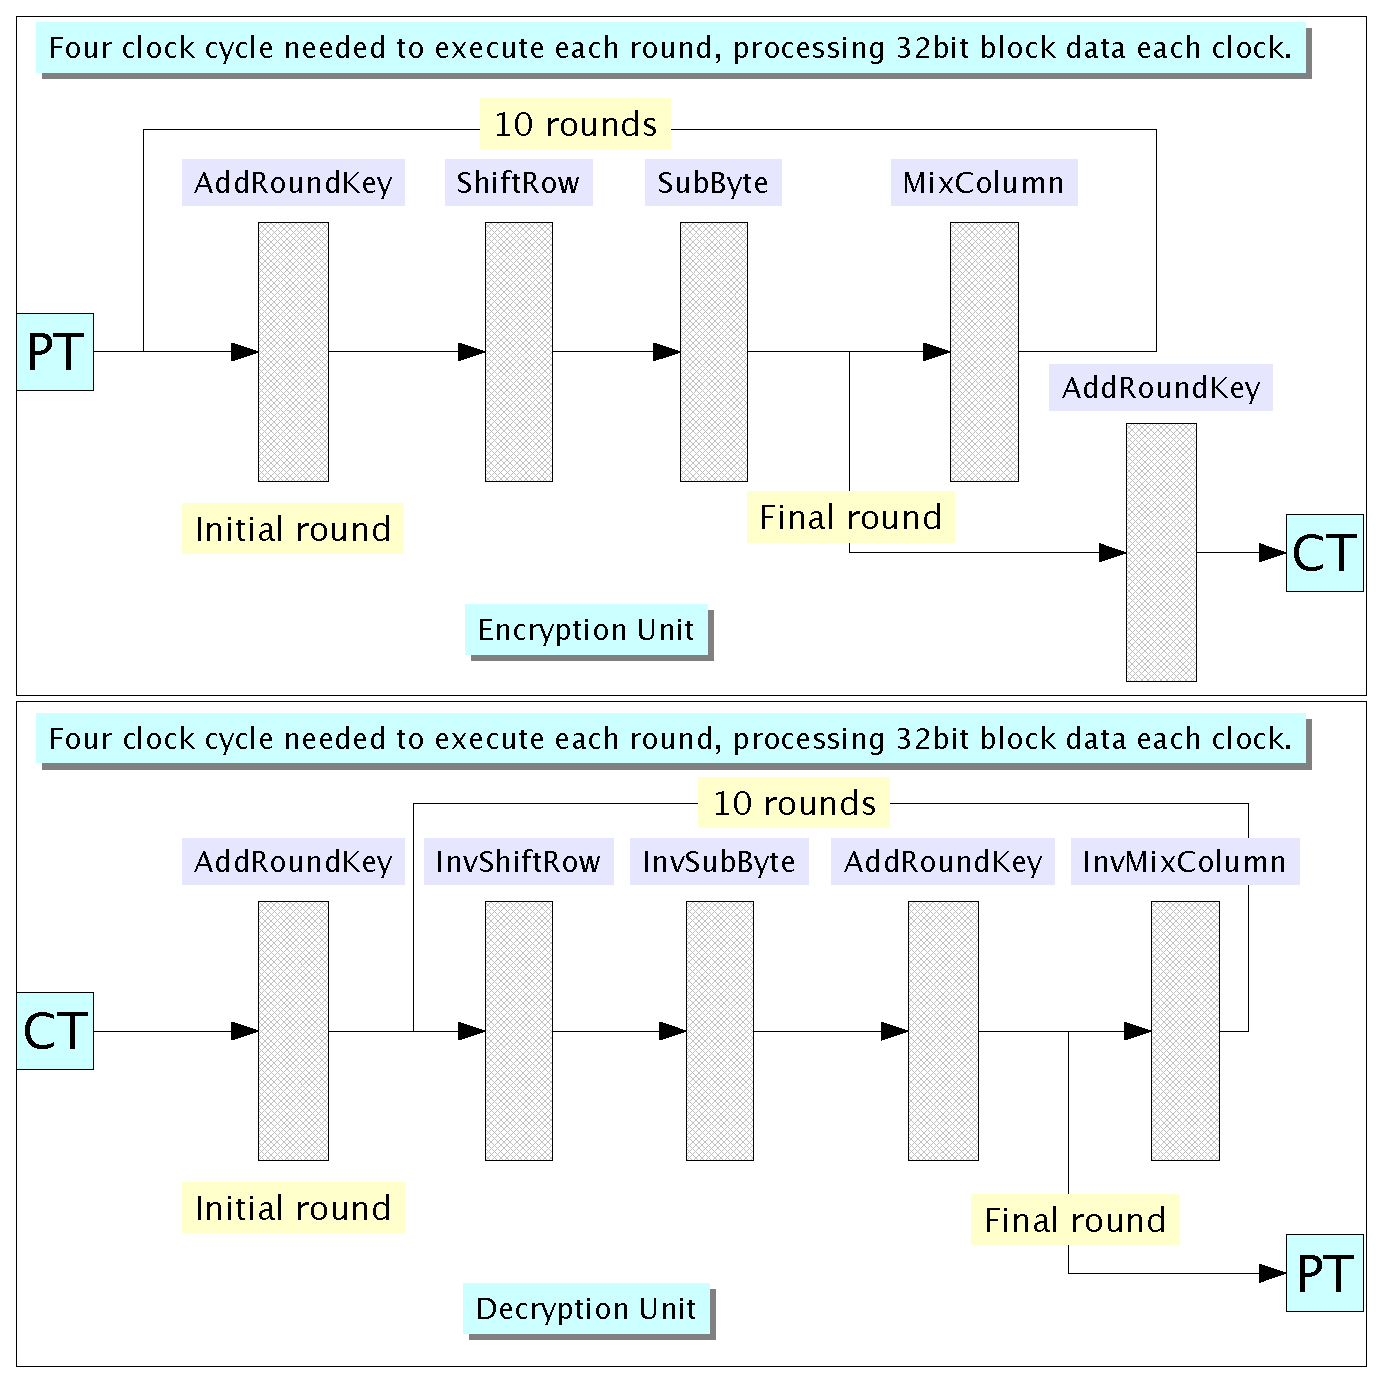
\includegraphics[width=15cm,height=10cm]{circuit_schematic.eps}
\caption{Circuit schematic}
\label{circuit_schematic}
\end{figure}

\section{Simulation}

Simulation is done by ModelSim 6.0 SE, the simulation is performed to
verify the correctness of design. The encryption and decrption units has
been verified using Electronic Codebook (ECB) method and passed 128 test
vector verification phase of Tables Known Answer Test (KAT).

\section{Synthesize}

This design has been synthesized using ISE Xilinx 6.3i, here is the
summary of the area utilization in FPGA Xilinx:

\begin{table}[H]
\center
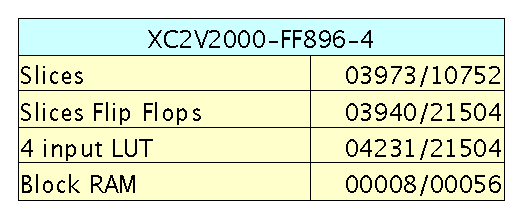
\includegraphics[width=8cm,height=2.5cm]{area.eps}
\caption{Area utilizations summary}
\label{area}
\end{table}

The maximum clock frequency is 50.594 MHz (Minimum period 19.765ns)

\section{Circuit Explanation}

\begin{figure}[H]
\center
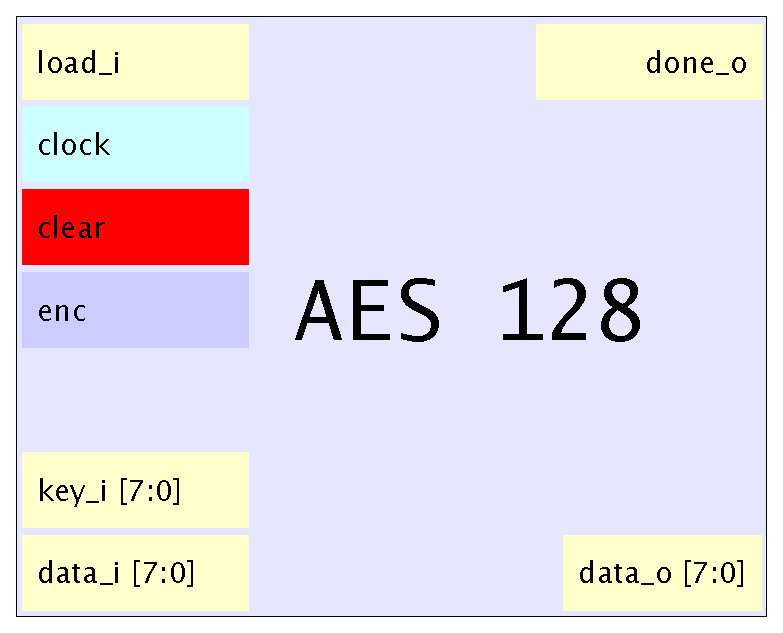
\includegraphics[width=5cm,height=4cm]{aes128block.eps}
\caption{AES 128 Input - Output Pin}
\label{aes128block}
\end{figure}

The AES 128 is composed from four subcircuit, these subcircuit are :
\begin{itemize}
\item ShiftRow
\item SubByte
\item MixColumn
\item KeyScheduler
\end{itemize}
%These subcircuit is the main component that build AES 128.

\subsection{ShiftRow}

ShiftRow transformation is performed by arranging the sequence of input
data to be processed, these transformation is performed this way:

\begin{displaymath}
\left\{
\begin{array}{lcl}
input    &    & output \\
0,5,a,f  & => & 0,1,2,3\\
4,9,e,3  & => & 4,5,6,7\\
8,d,2,7  & => & 8,9,a,b\\
c,1,6,b  & => & c,d,e,f\\
\end{array}
\right\}
\end{displaymath}

the InvShiftRow transformations operations is performed using the
following sequence of input data:

\begin{displaymath}
\left\{
\begin{array}{lcl}
input    &    & output \\
0,d,a,7  & => & 0,1,2,3\\
4,1,e,b  & => & 4,5,6,7\\
8,5,2,f  & => & 8,9,a,b\\
c,9,6,3  & => & c,d,e,f\\
\end{array}
\right\}
\end{displaymath}

\subsection{SubByte}

SubByte transformation is implemented using dedicated block RAM, SubByte
transformation occupy 4 Kb Block RAM in 512x8 configurations.

\subsection{MixColumn}

The MixColumn is implemented using matrix calculation of following equation:

\begin{equation}
c(x) =~'03'~x^3 +~'01'~x^2 +~'01'~x +~'02'.
\end{equation}

matrix form of above equation is:

\begin{displaymath}
\left[ \begin{array}{c} b_0\\ b_1\\ b_2\\ b_3\\ \end{array} \right]
=
\left[ \begin{array}{c} 02~03~01~01\\ 01~02~03~01\\ 01~01~02~03\\ 03~01~01~02\\ \end{array} \right]
\left[ \begin{array}{c} a_0\\ a_1\\ a_2\\ a_3\\ \end{array} \right]
\end{displaymath}

The InvMixColumn operations is performed using following equation:

\begin{equation}
d(x) =~'0b'~x^3 +~'0d'~x^2 +~'09'~x +~'0e'.
\end{equation}

in matrix representation is:

\begin{displaymath}
\left[ \begin{array}{c} d_0\\ d_1\\ d_2\\ d_3\\ \end{array} \right]
=
\left[ \begin{array}{c} 0e~0b~0d~09\\ 09~0e~0b~0d\\ 0d~09~0e~0b\\ 0b~0d~09~0e\\ \end{array} \right]
\left[ \begin{array}{c} c_0\\ c_1\\ c_2\\ c_3\\ \end{array} \right]
\end{displaymath}

The InvMixColumn can be implemented using resource sharing, by following
equation:

\begin{equation}
c(x) \otimes d(x) =~'01'
\end{equation}

then if we multiply both side with $d^2(x)$ then it become:

\begin{equation}
c(x) \otimes d^2(x) = d(x)
\end{equation}

above equation state that we can get the InvMixColumn  using
multiplication of MixColumn operations and $d^2(x)$:

\begin{equation}
d^2(x) =~'04'~x^2 +~'05'.
\end{equation}

and matrix representation of above equation is:

\begin{displaymath}
\left[ \begin{array}{c} e_0\\ e_1\\ e_2\\ e_3\\ \end{array} \right]
=
\left[ \begin{array}{c} 05~00~04~00\\ 00~05~00~04\\ 04~00~05~00\\ 00~04~00~05\\ \end{array} \right]
\left[ \begin{array}{c} c_0\\ c_1\\ c_2\\ c_3\\ \end{array} \right]
\end{displaymath}

\subsection{KeyScheduler}

The KeyScheduler is implemented using the following schematic diagram:

\begin{figure}[H]
\center
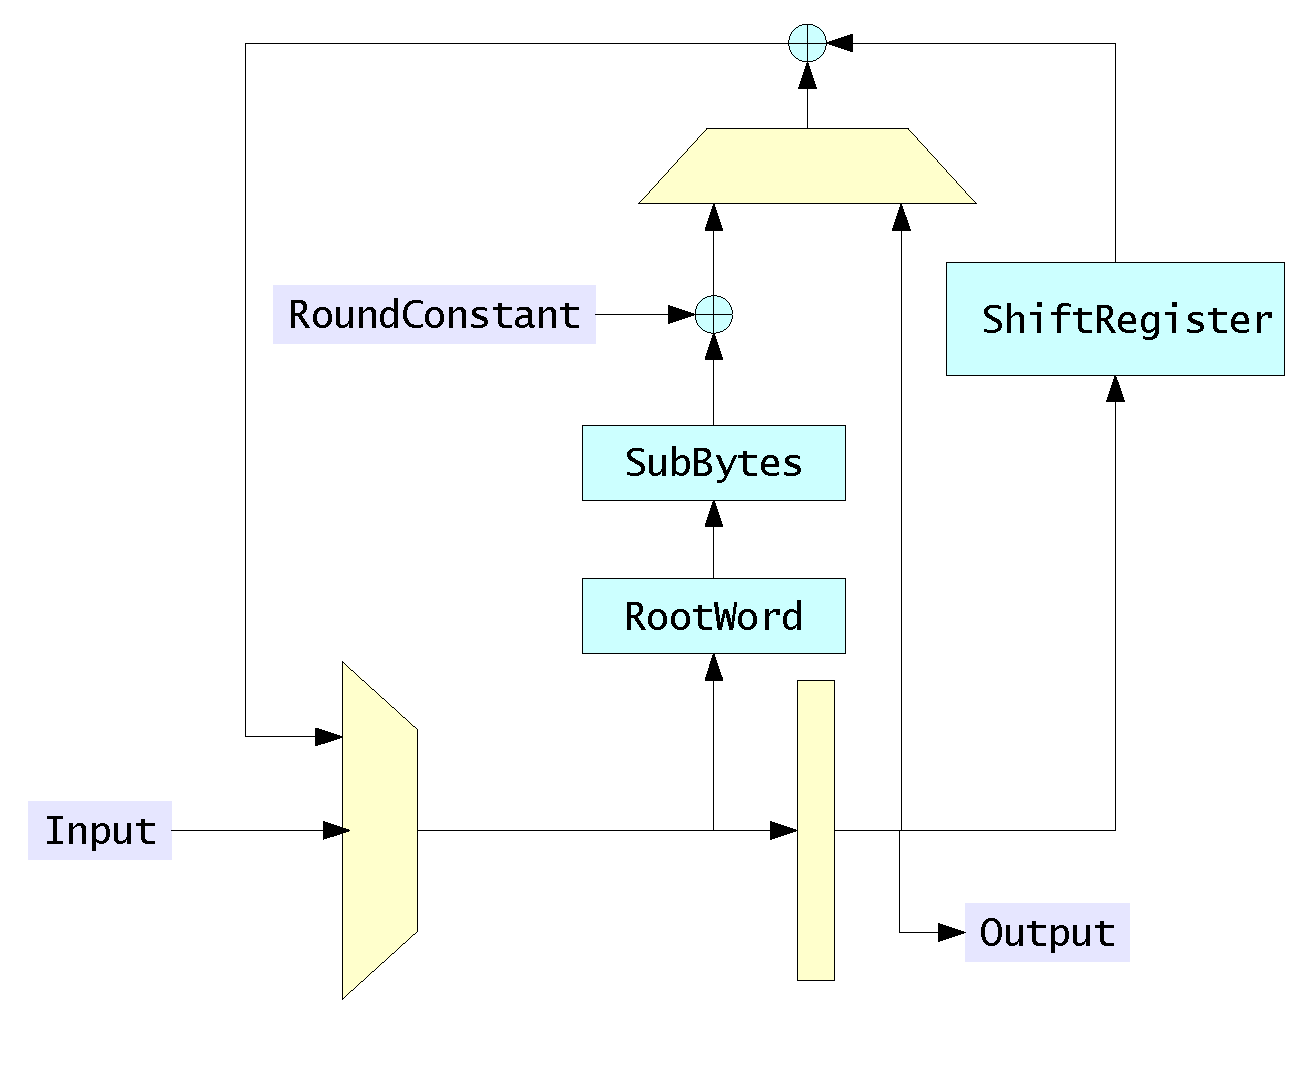
\includegraphics[width=9cm,height=6cm]{key_scheduler.eps}
\caption{KeyScheduler Schematics}
\label{key_scheduler}
\end{figure}

\section{TODO}

\begin{itemize}
%\item Finish decryption circuit.
\item Optimize Key Scheduler storage allocations implementations.
\item Optimize folded register implementation.
\item Implement TriState Buffer for switching SubBytes utilization.
\item Update documentation.
\item CleanUp code.
\end{itemize}

\begin{thebibliography}{1}

\bibitem{chodowiec}
Pawel Chodowiec and Kris Gaj, \textbf{Very Compact FPGA Implementation
of the AES Algorithm}, CHES 2003, LNCS 2779, pp. 319-333

\bibitem{fips197}
Federal Information Processing Standards Publication 197,
\textbf{Advanced Encryption Standard (AES)}, National Institute of
Standards and Technology, 2001.

\bibitem{rijndael}
Daemen J. and Rijmen V., \textbf{AES Proposal: The Rijndael Block Cipher},\\
\href{http://www.esat.kuleuven.ac.be/~rijmen/rijndael/Rijndael.pdf}{http://www.esat.kuleuven.ac.be/\~~rijmen/rijndael/Rijndael.pdf}

%\bibitem{wada}
%Tom Wada, \textbf{2-D Product Code Iterative Decoder},\\
%\href{http://www.ie.u-ryukyu.ac.jp/\~\ wada/design06/spec\_e.html}
%     {http://www.ie.u-ryukyu.ac.jp/\~\ wada/design06/spec\_e.html}\\
%     October 1$^{st}$, 2005

\end{thebibliography}

\appendix

\chapter{Informations}

\section{Tools}

\begin{itemize}
\item \textbf{ModelSim 6.0} The Simulator
\item \textbf{Xilinx 6.3i} The Synthesizer
\item \textbf{VIM} (Vi IMproved) / \textbf{Emacs} The Editor
\item \textbf{\LaTeX}~~The Typesetter
\item \textbf{OpenOffice.org 2.0} The Drawer
\end{itemize}

\vspace{1cm}
\begin{tabbing}
\textbf{Version: 1.0} 
\end{tabbing}

\end{document}
